\documentclass[12pt]{article}
\usepackage[utf8]{inputenc}
\usepackage{amssymb}
\usepackage{amsthm}
\usepackage{amsmath}
\usepackage[margin=0.75in]{geometry}
\usepackage{enumitem}
\usepackage{graphicx}
\usepackage{indentfirst}

\newcommand{\bi}[1]{\mbox{\textbf{#1}}}

\author{Creating a Neural Network\bigskip\\Athena Boose}
\title{Math 225 Applications Project}
\date{\today}

\begin{document}
\maketitle

\textbf{Bolded} terms are defined in the Glossary at the end.
If you are only interested in the linear algebra of this project, skip to section 2.

\section{Design Decisions}

\subsection{Overview}

My project involved creating a Neural Network to recognize handwritten digits.
My code is available under the MIT License at \verb|https://github.com/chickenspaceprogram/digit-recognizer|.
Windows builds are currently not supported, although it is possible that they will be in future when I get more time.
It should be functioning on MacOS and Linux (although for Linux it is possible you may have to configure a few things; if building fails, email me with the distribution you're using and I can help troubleshoot).

\subsection{Programming Language Selection and General Philosophy}

I opted to not use any external machine learning libraries, as I wanted to gain as much experience with the algorithms and math behind neural networks as possible.
However, I did use the \textbf{BLAS library} to handle things like matrix-vector multiplication, dot products, and vector addition.
Everything else was coded manually.

I chose to code this project in C++.
I opted to use C++ rather than C, as it seemed sensible to represent the layers of the neural network and the network itself as objects.
I opted for C++ over something like Fortran as I have more experience in C-style languages and was running low on time.
C++ is also likely to run faster than something like Java or Python.

\subsection{Structure}

This program is structured in several parts. 
First, there are the library functions I created.
These are located in the directory \verb|src/libs/|, and they handle interfacing with BLAS (which has an awkward interface), loading the images from files, and generating random numbers.

Second, there are the files in \verb|src/network/|, which handle most of the logic of the neural network.
In this folder, code describing the activation functions of each layer and the cost function of the network are described.
Also, objects representing a single layer of the neural network as well as the entire network are described.

Finally, in the main \verb|src/| folder, the functions specific to training the network to recognize handwritten digits are located.
\verb|src/train.cpp| handles interfacing with the code in \verb|src/network/|, and \verb|src/test-net.cpp| checks to see how many of the test files the network recognizes correctly.
\verb|src/main.cpp| handles configuring the network and running it.

The \verb|build/| directory handles the \textbf{CMake} configuration for the Release build, and \verb|debug/| has the configurations for the debugging build.
The \verb|mnist-dataset/| directory contains the images from the MNIST dataset.

\section{Algorithm}

Neural networks are composed of many layers, each composed of nodes.
The first layer is called the input layer, and it contains nodes with activations representing the input data.
The last layer is called the output layer, and it contains nodes with activations representing the network's output.
The layers in between the input and output are called hidden layers.
Each node has an activation, which is a scalar value describing how strongly the input activated it.
This means that each layer can be written as a vector containing each node's activation.

The activation of node $j$ in layer $i$ is described as follows (please note that superscripts do not denote exponents here):

\[
a_j^i = f\left(b_j^i + \sum_{k = 1}^{m} a_k^{i-1} \cdot w_{jk}^i\right)
\]

where $b_j^i$ is a scalar bias added to the $j$th node in the $i$th layer, $a_k^{i-1}$ is the $k$th node in the $i-1$th layer, $w_{jk}^i$ is the weight between node $a_k^{i-1}$ and node $a_j^i$, and $f$ is some nonlinear \textbf{activation function}.
The goal of a neural network is to tune the weights and biases of all the nodes to produce a desired output.
This can be rewritten as follows:

\[
\bi{a}^i = f\left(\bi{b}^i + W^i\bi{a}^{i-1}\right)
\]

where $\bi{a}^i$ is a vector containing the activations of layer $i$, $f$ is a function that returns a vector and applies the activation function to every element of its input, $\bi{b}^i$ is a vector containing the biases of layer $i$, $W^i$ is a matrix containing the weights from layer $i - 1$ to $i$, and $\bi{a}^{i-1}$ is the activations of layer $i - 1$.

Calculating how to adjust the weights and biases of a network to produce a desired output is the job of the backpropagation algorithm.
Very roughly, a ``cost function'' is used to assign a scalar value to the amount that the output layer differs from the desired output.
Then, the gradient of this cost function with respect to all the weights and biases of the network is determined, and this gradient is used to adjust these weights and biases in the correct direction to make the cost function's value decrease.

A full explanation of that algorithm is outside the scope of this discussion as it is at best tangential to the usage of linear algebra in this project.
However, it will be noted that the error at a specific layer $i-1$ of the network (a value important for calculating the gradient of the cost function) can be recursively described as:

\[
\delta^{i-1} = (f^{i-1})'\left(\left(W^i\right)^T\delta^i\right)
\]

where $\delta^{i-1}$ is a vector representing the error at layer $i - 1$, $(f^{i-1})'$ is the derivative of the activation function, $W^i$ is the matrix of weights at layer $i$, and $\delta^i$ is the error at layer $i$.

\bigskip

It is beneficial to describe these equations in terms of matrix-vector multiplication and vector addition to enable the usage of linear algebra libraries.
These libraries are code written by other people that take advantage of various optimizations to compute matrix-vector products faster than can usually be done when writing code by hand.

\section{Figures}

\begin{center}
    \begin{figure}[h!]
        \caption{
            This graph shows the number of images out of the 10000-image set of test cases that the neural network recognized correctly.
            As the number of iterations increases, the network is able to recognize more and more images correctly from the test set.
            The network is not perfect, and tends to plateau at getting roughly 90\% of the images correct with these parameters. 
            I think that with some tweaking to the parameters used and with using a more-annoying-to-implement but better cost function, this number could be brought higher.
            As well, I suspect that there are a few lingering bugs in my code potentially reducing the network's efficiency, however I did not have time to search for and fix these.
            \smallskip
        }
        \centering
        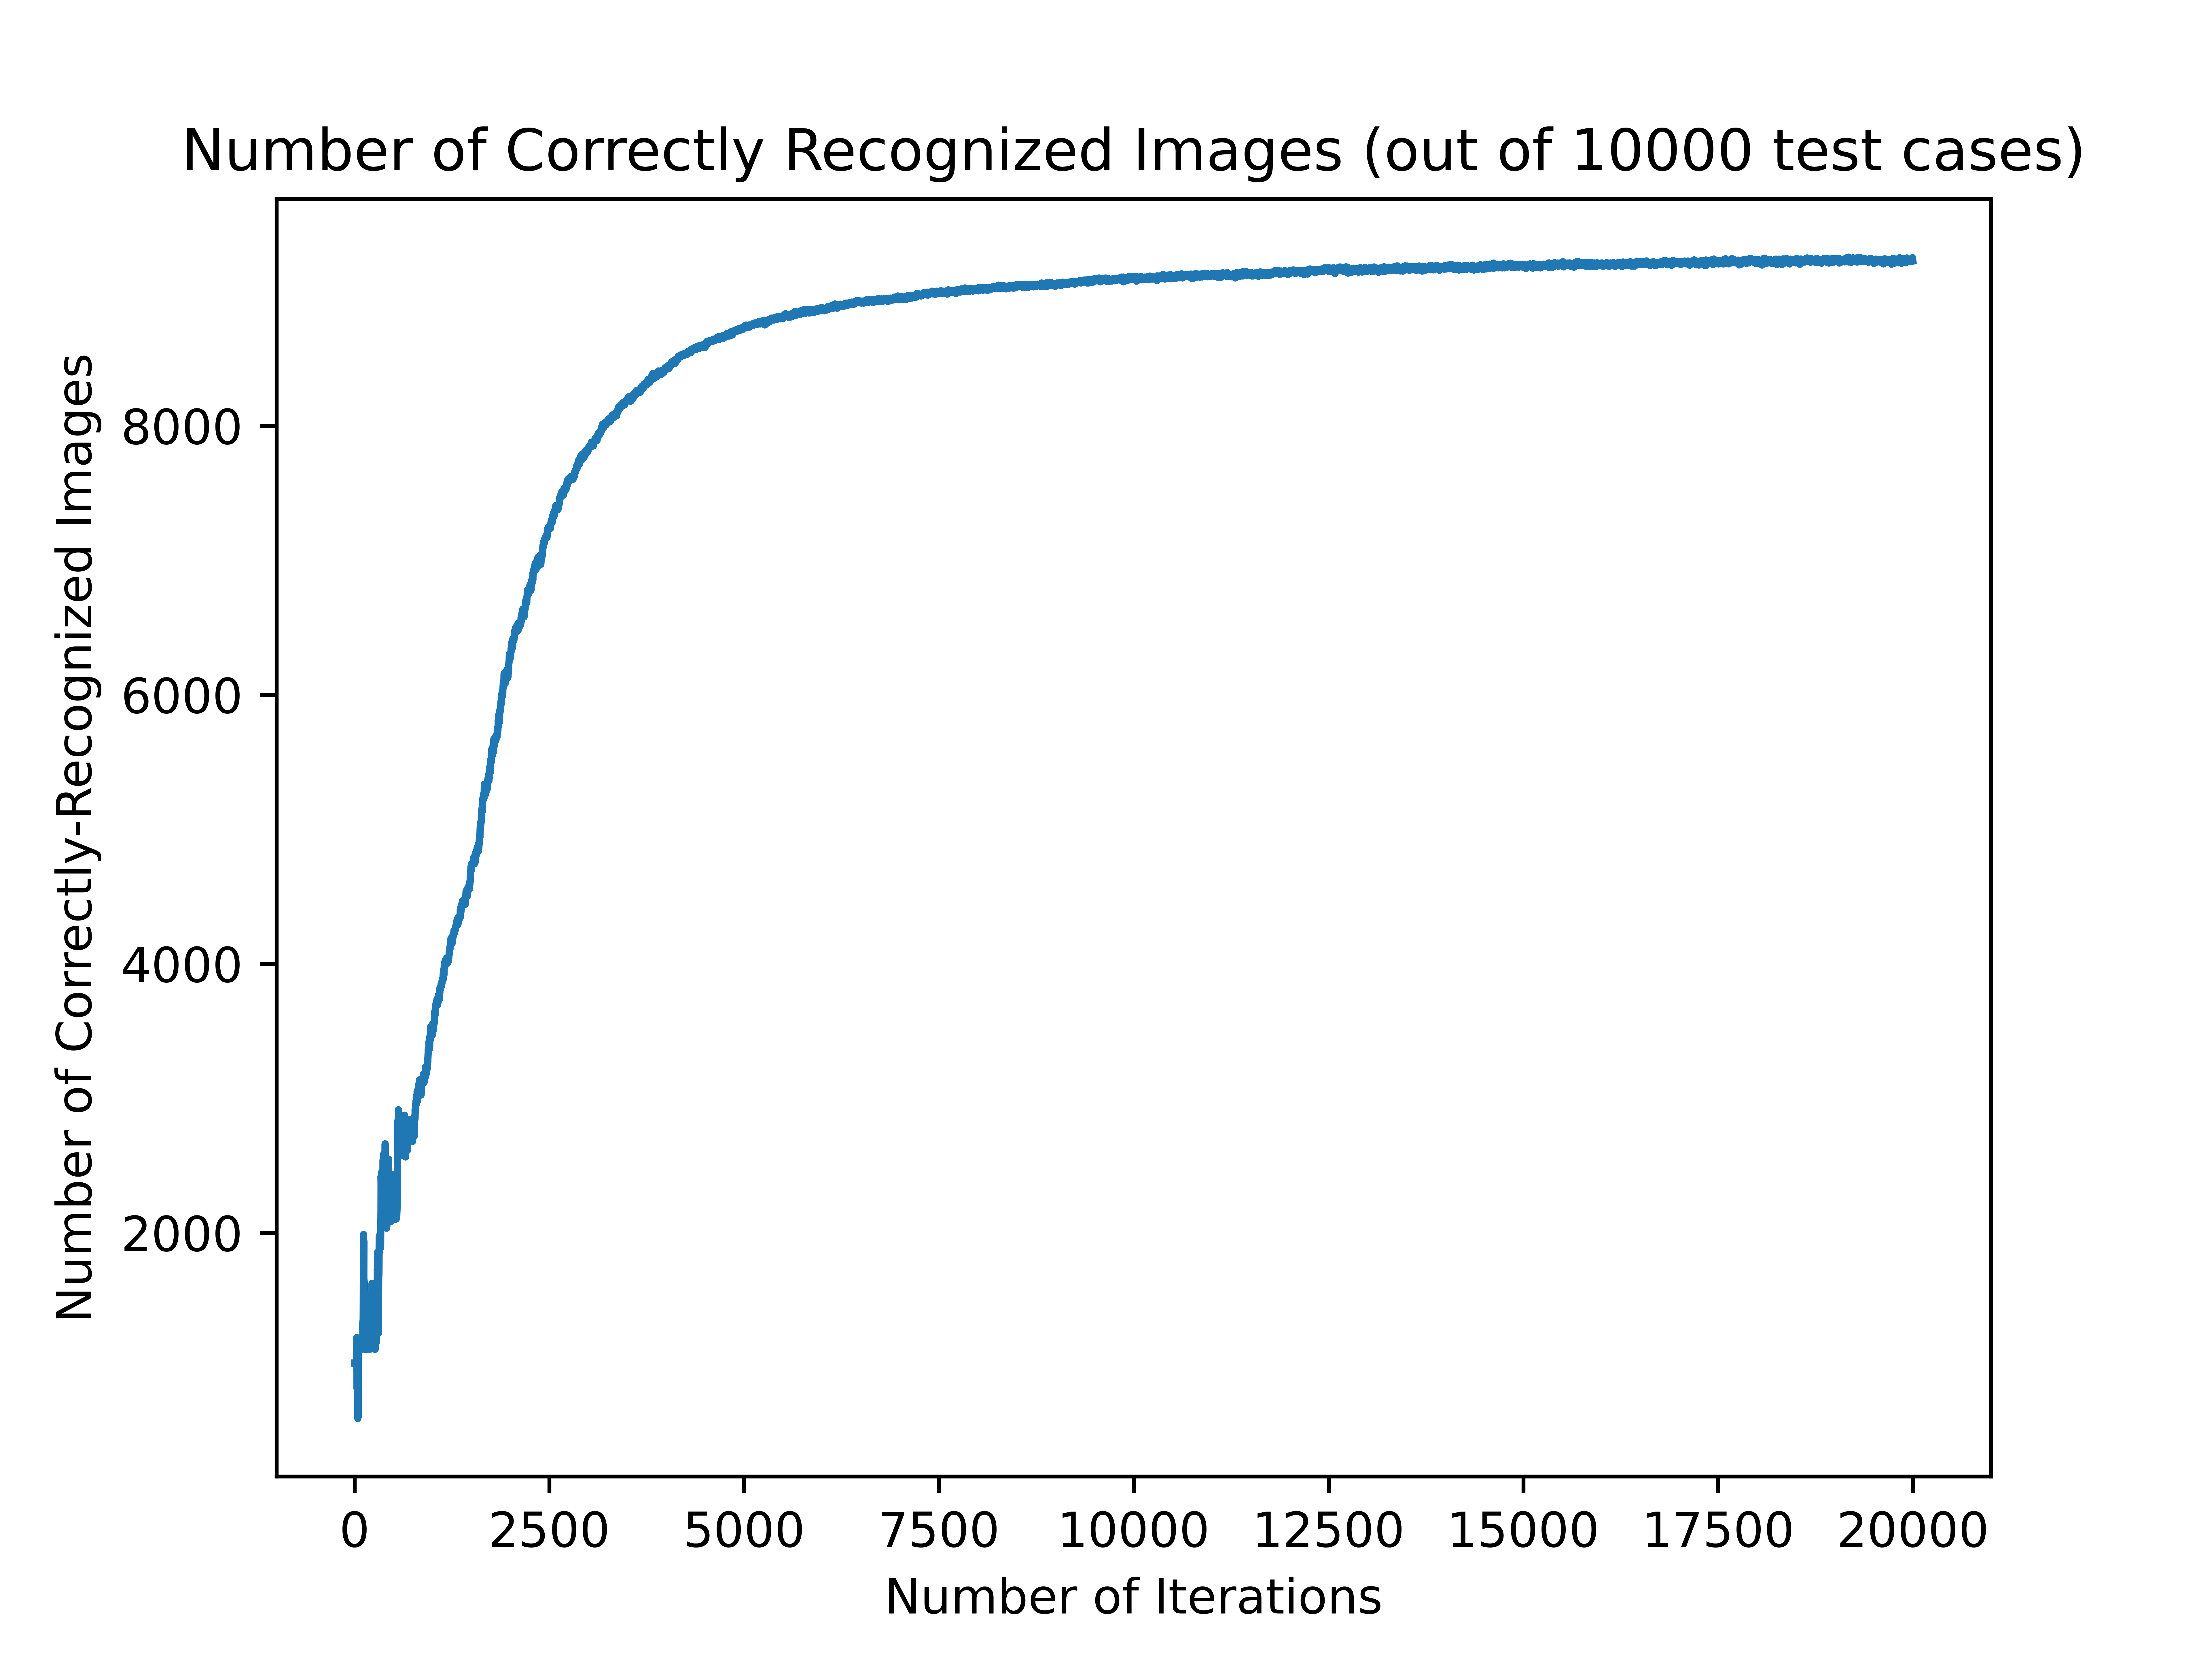
\includegraphics[scale=0.9]{test-2layer-10node-act0.3-2/network.png}

        Parameters used:
        \medskip
        \begin{itemize}
            \itemsep0em 
            \item 2 hidden layers
            \item 10 nodes in hidden layers
            \item Learning rate: 0.1
            \item Batch size: 500
            \item Image activations normalized to values from 0 to 1
            \item Network weights initialized to random numbers from -0.3 to 0.3
            \item Network biases initialized to 0 
        \end{itemize}
        \centering
    \end{figure}
\end{center}

\section{Glossary}

\begin{itemize}
    \item \textbf{MNIST dataset} - 
    A set of 70000 images of handwritten digits, divided into 60000 images used for training a neural network and 10000 images for testing it. 
    The dataset is available at \verb|https://yann.lecun.com/exdb/mnist/|, although the website is a bit broken. 
    \item \textbf{BLAS} - 
    A definition of various linear algebra subroutines for things like matrix-matrix multiplication, matrix-vector multiplication, dot products, vector addition, and other things.
    Various implementations of BLAS exist, notably OpenBLAS for Windows and Linux and the one in Apple's Accelerate framework for MacOS.
    \item \textbf{CMake} -
    A build system for C and C++ programs.
    It figures out how to link the code in the files of this project (essentially it makes the code in the different files of this project all interface together in the correct way).
    \item \textbf{Activation Function} - 
    A nonlinear function applied to the weights of a neural network.
    This function prevents the entire network from being equivalent to some linear transformation.
    Common activations are the ReLU (which equals its input if the input is $>$ 0 and equals 0 otherwise) and the logistic function $\frac{e^x}{1+e^x}$.
\end{itemize}

\end{document}